\section{Results}\label{sec:results}
We now present our $\fnl$ constraints obtained from the power spectrum of the DESI LRG targets. The treatment of the imaging systematic effects is performed on each imaging region (BASS+MzLS, DECaLS North/South) separately. After cleaning, the regions are combined for the measurement of the power spectrum. We unblind the galaxy power spectrum and the $\fnl$ values after our cleaning methods are validated and vetted by the cross power spectrum and mean galaxy density diagnostics. We also conduct additional tests to check the robustness of our constraints against various assumptions, such as analyzing each region separately, applying cuts on imaging conditions, and changing the smallest mode used in fitting for $\fnl$.

\subsection{DESI imaging LRG sample}
\begin{figure}
    \centering
    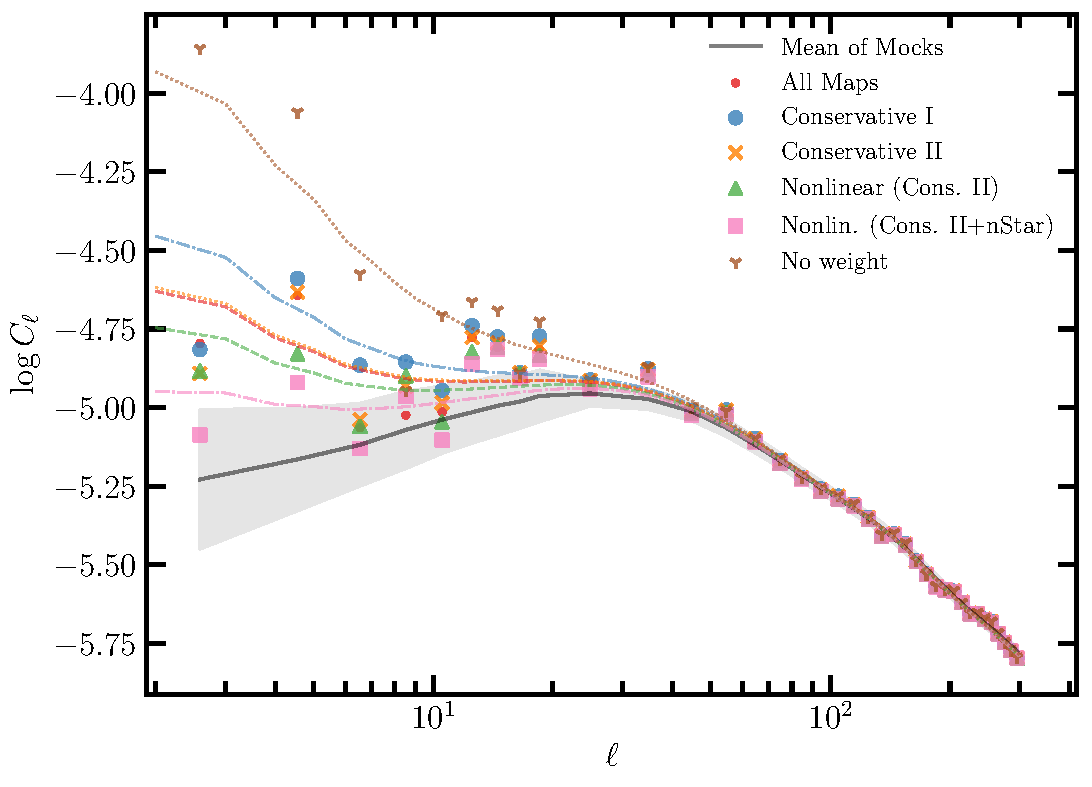
\includegraphics[width=0.47\textwidth]{figures/model_dr9.pdf} 
    \caption{The angular power spectrum of the DESI LRG targets before (\textit{No weight}) and after correcting for imaging systematics using the \mout{linear and} non-linear method \mr{with various combinations of maps}. The curves represent the corresponding best-fitting theory predictions. The solid curve and grey shade respectively represent the mean power spectrum and $68\%$ error from the $\fnl=0$ mocks. \mr{We associate the differences on modes $\ell < 20$ to over-correction.}}
    \label{fig:cl_dr9}
\end{figure}
We find that the excess clustering signal in the power spectrum of the DESI LRG targets is mitigated after correcting for the imaging systematic effects. Figure \ref{fig:cl_dr9} shows the measured power spectrum of the DESI LRG targets before and after applying imaging weights and the best-fitting theory curves. The solid grey line and the grey shade represent respectively the mean power spectrum and 1$\sigma$ error, estimated from the $\fnl=0$ lognormal simulations. The differences between various cleaning methods are significant on large scales ($\ell < 20$), but the small scale clustering measurements are consistent. \mr{We associate the differences to over-correction caused by including more maps for the treatment of systematics.} \mout{By comparing \textit{linear two maps} to \textit{linear three maps}, we find that the measured clustering power on modes with $6\leq \ell < 10$ are noticeably different between the two methods. We associate the differences to the additional map for psfsize in the r-band, which is included in \textit{linear three maps}. On other scales, the differences between \textit{linear three maps} and \textit{linear eight maps} are negligible, supporting the idea that our feature selection procedure has been effective in identifying the primary maps which cause the large-scale excess clustering signal. Comparing \textit{non-linear three maps} to \textit{linear three maps}, we find that the measured spectra on $4 \leq \ell < 6$ are very different, probably indicating some non-linear spurious fluctuations with large scale characteristics due to extinction.} \mr{Comparing \textit{non-linear three maps} to \textit{non-linear four maps}, we find that} adding stellar density in the non-linear approach (\textit{non-linear four maps}) further reduces the excess power relative to the mock power spectrum, in particular on modes between $2\leq \ell < 4$. However, when calibrated on the lognormal simulations, we find that the over-subtraction due to stellar density is reversed after accounting for over-correction.


\subsubsection{Calibrated constraints}

\begin{figure}
    \raggedleft
    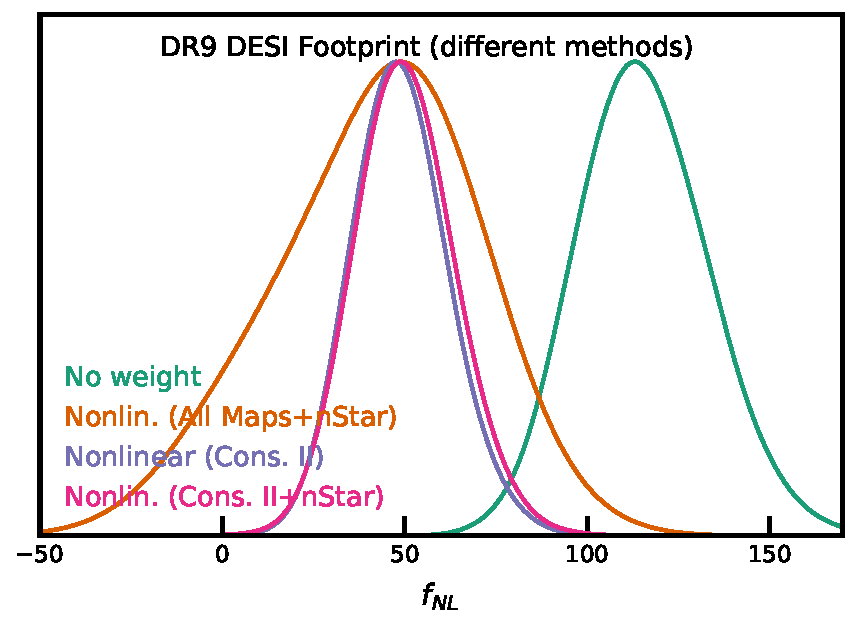
\includegraphics[width=0.439\textwidth, trim={0 1.4cm 0 0},clip]{mcmc_dr9methods1d.pdf}
    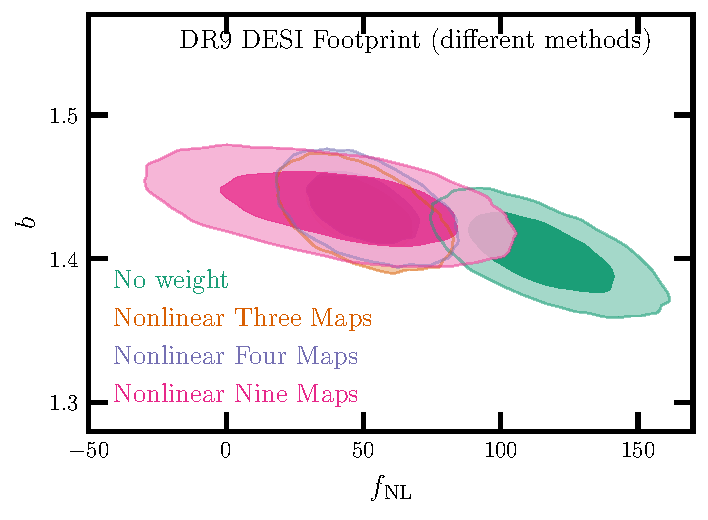
\includegraphics[width=0.47\textwidth, trim={0 0 0.15cm 0.2cm},clip]{figures/mcmc_dr9methods.pdf} 
    \caption{The calibrated constrains from the DESI LRG targets. \textit{Top}: probability distribution for $\fnl$ marginalized over the shotnoise and bias. \textit{Bottom}: $68\%$ and $95\%$ probability distribution contours for the bias and $\fnl$ from the DESI LRG targets before and after applying non-linear cleaning methods. The lognormal mocks are used to calibrate these distributions for over-correction.}\label{fig:mcmc_dr9}
\end{figure}

\begin{figure}
\raggedleft
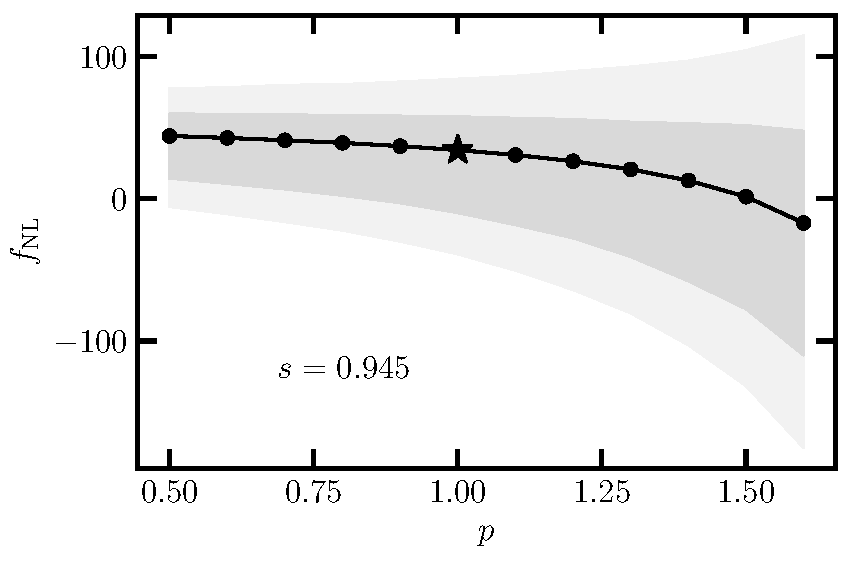
\includegraphics[width=0.45\textwidth]{figures/fnl_p.pdf}
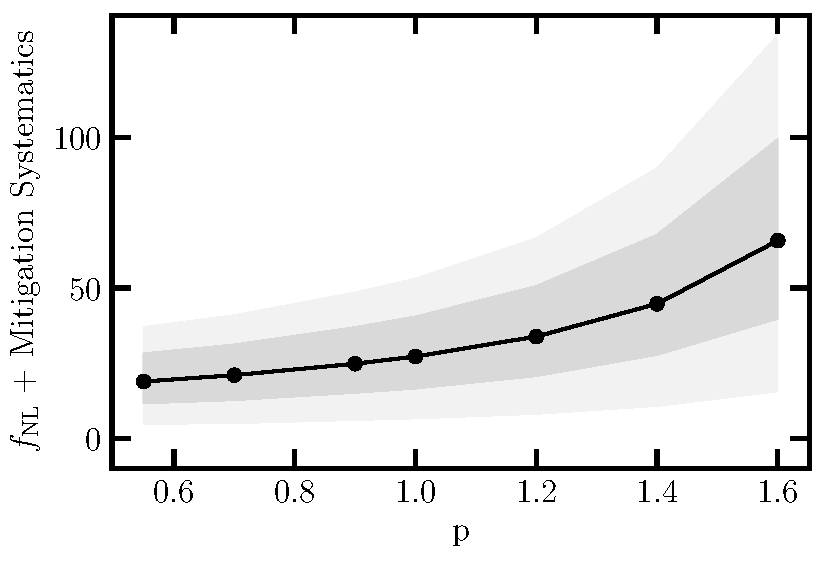
\includegraphics[width=0.437\textwidth]{figures/fnl_magbias.pdf}
\caption{\mr{The best-fitting estimates of $\fnl$ and their corresponding $68\%$ ($95\%$) errors from the DESI LRG targets using the non-linear nine maps approach under various values of $p$ or $s$. The star symbol represents the fiducial analysis with $p=1$ and $s=0.945$.}}\label{fig:fnl_magbias}
\end{figure}

\begin{table*}
    \caption{The calibrated best-fitting, marginalized mean, and marginalized $68\%$ ($95\%$) confidence estimates for $\fnl$ from fitting the power spectrum of the DESI LRG targets before and after correcting for imaging systematic effects. The lowest mode is $\ell_{\rm min}=2$\mr{, $p=1$, and $s=0.945$.}}
    \label{tab:dr9methodcalib}
   \centerline{%     
    \begin{tabular}{llllllll}
    \hline
    \hline
   &  & 	  & & $\fnl$ &  &  \\
   \cmidrule(r{.7cm}){3-6}
Footprint      & Method & 	Best fit  & Mean & $ 68\%$ CL & $ 95\%$ CL & $\chi^{2}$ (dof=$34$) \\
    \hline
DESI & No Weight                        & $   118$& $   121$& $   102<\fnl<   140$& $    86<\fnl<   161$ &   45.1\\
DESI & Nonlinear Three Maps             & $    46$& $    47$& $    33<\fnl<    61$& $    21<\fnl<    76$ &   33.9\\
DESI & Nonlinear Four Maps              & $    46$& $    47$& $    33<\fnl<    62$& $    19<\fnl<    78$ &   34.4\\
DESI & Nonlinear Nine Maps              & $    34$& $    24$& $   -10<\fnl<    58$& $   -39<\fnl<    84$ &   39.1\\    
   \hline
    \end{tabular}
}
\end{table*}

All $\fnl$ constraints presented here are calibrated for the effect of over-correction using the lognormal simulations. Table \ref{tab:dr9methodcalib} describes the best-fitting and marginalized mean estimates of $\fnl$ from fitting the power spectrum of the DESI LRG targets before and after cleaning with the non-linear approach given various combinations for the imaging systematic maps. Figure \ref{fig:mcmc_dr9} shows the marginalized probability distribution for $\fnl$ in the top panel, and the $68\%$ and $95\%$ probability contours for the linear bias parameter and $\fnl$ in the bottom panel, from our sample before and after applying various corrections for imaging systematics. Overall, we find the maximum likelihood estimates to be consistent among the various cleaning methods. We obtain \mr{$33 (21) < \fnl < 61(76)$} at $68\%(95\%)$ confidence with \mr{$\chi^{2}=33.9$} for \textit{non-linear three maps} with $34$ degrees of freedom. Accounted for over-correction, we obtain \mr{$33(19) < \fnl < 62(78)$ with $\chi^{2}=34.4$ using \textit{non-linear four maps} which includes the additional stellar density map}. With or without stellar density, the confidence intervals are consistent with each other and significantly off from zero PNG; specifically, the probability that $\fnl$ is greater than zero, $P(\fnl >0)=99.9$ per cent. We also apply a more aggressive systematics treatment that includes regression using the non-linear approach against the full set of imaging maps we identified, non-linear nine maps, and find that \mr{zero $\fnl$ is recovered. Specifically,} our maximum
likelihood value changes \mout{only slightly} to \mr{$\fnl \sim 34$ with $\chi^{2}=39.1$}, \mout{but} \mr{and uncertainty on $\fnl$ expands, resulting in a range of $-10 (-39) < \fnl < 58 (84)$ at $68\% (95\%)$ confidence. This increase is attributed to the aggressive treatment, which removes large-scale clustering information and diminishes the constraining power of the dataset. Additionally, we explore the sensitivity of the $\fnl$ posterior using the non-linear nine maps method while varying the values of $p$ in the range of $0.5$ to $1.6$ and $s$ in the range of $0.75$ to $1.25$. Figure \ref{fig:fnl_magbias} illustrates our findings, and Table \ref{tab:dr9ps} provides a summary. Regardless of the values chosen for $p$ and $s$, we reliably recover $\fnl=0$ within the $95\%$ confidence interval.} For comparison, we obtain \mr{$102(86) < \fnl < 140(161)$} at $68\% (95\%)$ confidence with \mr{$\chi^{2}=45.1$} for the \textit{no weight} case.

\begin{table*}
    \caption{\mr{The calibrated best-fitting, marginalized mean, and marginalized $68\%$ ($95\%$) confidence estimates for $\fnl$ from the DESI LRG targets after non-linear nine maps and various values of $p$ and $s$.}}
    \label{tab:dr9ps}
   \centerline{%     
    \begin{tabular}{llllll}
    \hline
    \hline
   &  & 	  & $\fnl$ &  &    \\
   \cmidrule(r{.7cm}){2-5}
Parameter & 	Best fit  & Mean & $ 68\%$ CL & $ 95\%$ CL & $\chi^{2}$ (dof=$34$) \\
\hline
$p=$ 0.5                                     & $    44$& $    37$& $    14<\fnl<    60$& $    -6<\fnl<    77$ &   39.1\\
0.6                                     & $    43$& $    35$& $    11<\fnl<    59$& $   -11<\fnl<    78$ &   39.1\\
0.7                                     & $    41$& $    33$& $     7<\fnl<    59$& $   -16<\fnl<    80$ &   39.1\\
0.8                                     & $    39$& $    31$& $     2<\fnl<    58$& $   -22<\fnl<    80$ &   39.1\\
0.9                                     & $    37$& $    28$& $    -3<\fnl<    58$& $   -30<\fnl<    82$ &   39.1\\
1.0                                     & $    34$& $    24$& $   -10<\fnl<    58$& $   -39<\fnl<    84$ &   39.1\\
1.1                                     & $    31$& $    19$& $   -18<\fnl<    57$& $   -50<\fnl<    86$ &   39.1\\
1.2                                     & $    26$& $    15$& $   -28<\fnl<    56$& $   -64<\fnl<    89$ &   39.1\\
1.3                                     & $    21$& $     7$& $   -41<\fnl<    54$& $   -80<\fnl<    93$ &   39.0\\
1.4                                     & $    13$& $    -2$& $   -58<\fnl<    53$& $  -103<\fnl<    97$ &   39.0\\
1.5                                     & $     1$& $   -13$& $   -77<\fnl<    51$& $  -131<\fnl<   104$ &   39.0\\
1.6                                     & $   -17$& $   -31$& $  -110<\fnl<    47$& $  -175<\fnl<   114$ &   39.0\\
\hline
$s=$ 0.75                                    & $    42$& $    31$& $    -1<\fnl<    62$& $   -30<\fnl<    87$ &   39.2\\
0.80                                    & $    40$& $    30$& $    -3<\fnl<    61$& $   -32<\fnl<    86$ &   39.1\\
0.85                                    & $    38$& $    28$& $    -6<\fnl<    60$& $   -35<\fnl<    86$ &   39.1\\
0.90                                    & $    36$& $    26$& $    -8<\fnl<    58$& $   -36<\fnl<    84$ &   39.1\\
0.945                                   & $    34$& $    24$& $   -10<\fnl<    58$& $   -39<\fnl<    84$ &   39.1\\
1.00                                    & $    31$& $    22$& $   -13<\fnl<    56$& $   -42<\fnl<    83$ &   39.0\\
1.05                                    & $    28$& $    19$& $   -15<\fnl<    54$& $   -45<\fnl<    81$ &   39.0\\
1.10                                    & $    23$& $    17$& $   -18<\fnl<    52$& $   -48<\fnl<    80$ &   39.0\\
1.15                                    & $    17$& $    15$& $   -21<\fnl<    51$& $   -50<\fnl<    80$ &   38.9\\
1.20                                    & $     8$& $    12$& $   -24<\fnl<    48$& $   -53<\fnl<    77$ &   38.9\\
1.25                                    & $     3$& $     9$& $   -27<\fnl<    46$& $   -56<\fnl<    76$ &   38.8\\
    \end{tabular}}
\end{table*}

\subsubsection{Uncalibrated constraints: robustness tests}
Figure \ref{fig:mcmcdr9noshift} shows the probability distributions of $\fnl$ for various treatments before accounting for the over-correction effect. The method with the largest flexibility and more number of imaging systematic maps is more likely to regress out the clustering signal aggressively and return biased $\fnl$ constraints. \mr{While reporting the uncalibrated constraints, we therefore include the label `Mitigation Systematics' to emphasize that the $\fnl$ values will be subject to an unknown bias caused by over-correction}. \mout{As expected, non-linear nine maps yields the smallest maximum likelihood estimate of \mr{$\fnl=-13$}}. Our non-linear three maps returns a best-fitting estimate of \mr{$\fnl=27$} with the $68\%(95\%)$ confidence of \mr{$17(6)<\fnl <40(53)$} and \mr{$\chi^{2}=33.9$}. With the stellar density map included, non-linear four maps yields a smaller best-fitting estimates of \mr{$\fnl=14$} with the error of \mr{$5(-6)<\fnl<26(38)$}. The non-linear nine maps gives an \mr{asymmetric} posterior with the marginalized mean \mr{$\fnl=-17$}, \mr{and the smallest best-fitting} estimate \mr{of $\fnl=-13$} with the error of \mr{$-31(-44)<\fnl<-3(9)$}. \mr{The disparities in the best-fitting estimates can be linked to over-correction, mirroring the effects observed in the mocks (refer to Figure \ref{fig:contmcmc}). Consequently, caution is advised when considering the uncalibrated values. Without adjusting for over-correction, non-linear four maps and non-linear nine maps recover zero $\fnl$ within $95\%$ and $68\%$ confidence, respectively. However, the non-linear method with three maps exhibits tension with $\fnl=0$ at a confidence level of $99.5$ percent.}

\begin{table*}
    \caption{The uncalibrated best-fitting and marginalized mean estimates for $\fnl$ from fitting the power spectrum of the DESI LRG targets before and after correcting for systematics. The estimates are not calibrated for over-correction, and thus are subject to mitigation systematics. The number of degrees of freedom is 34 (37 data points - 3 parameters). The lowest mode is $\ell=2$\mr{, $p=1$,} and the covariance matrix is from the $\fnl=0$ clean mocks (no mitigation) except for the case with '+ Cov' in which the covariance matrix is from the $\fnl=76.9$ clean mocks (no mitigation). \mr{We fix $s=0.945$ for DESI, $0.943$ for DECaLS North (and South), and $0.951$ for BASS+MzLS.}}
    \label{tab:dr9method}
   \centerline{%     
    \begin{tabular}{llllllr}
    \hline
    \hline
   &  & 	&   &  $\fnl$ + Mitigation Systematics &  &  \\
   \cmidrule(r{.7cm}){3-6}
Footprint                               & Method & 	Best fit  & Mean & $ 68\%$ CL & $ 95\%$ CL & $\chi^{2}$ (dof=$34$) \\
    \hline
\bf{DESI} & \bf{No Weight}                        & $   \bf{118}$& $   \bf{121}$& $   \bf{102}<\fnl<   \bf{140}$& $    \bf{86}< \fnl<   \bf{161}$ &   \bf{45.1}\\
DESI & Linear Three Maps                & $    36$& $    37$& $    25<\fnl<    50$& $    14<\fnl<    64$ &   38.6\\
DESI & Linear Four Maps                 & $    31$& $    32$& $    20<\fnl<    45$& $     9<\fnl<    58$ &   40.3\\
\bf{DESI} & \bf{Linear Nine Maps}                 & $    \bf{30}$& $    \bf{32}$& $    \bf{19}<\fnl<   \bf{43}$& $     \bf{9}<\fnl<  \bf{57}$ &   \bf{41.9}\\
DESI & Nonlinear Three Maps             & $    27$& $    28$& $    17<\fnl<    40$& $     6<\fnl<    53$ &   33.9\\
DESI & Nonlinear Four Maps              & $    14$& $    15$& $     5<\fnl<    26$& $    -6<\fnl<    38$ &   34.4\\
\bf{DESI} & \bf{Nonlinear Nine Maps}              & $   \bf{-13}$& $   \bf{-17}$& $   \bf{-31}<\fnl<    \bf{-3}$& $   \bf{-44}<\fnl<     \bf{9}$ &  \bf{39.1}\\
DESI (imag. cut) & Nonlinear Nine Maps  & $   -25$& $   -22$& $   -37<\fnl<    -7$& $   -49<\fnl<     6$ &   37.7\\
DESI (comp. cut) & Nonlinear Nine Maps  & $   -24$& $   -23$& $   -35<\fnl<   -10$& $   -46<\fnl<     2$ &   36.3\\
DESI & Nonlinear Nine Maps+$f_{\rm NL}=76.9$ Cov& $   -11$& $   -15$& $   -30<\fnl<    0$& $   -43<\fnl<    12$ &   37.4\\
   \hline
BASS+MzLS & Nonlinear Three Maps        & $    13$& $    16$& $    -6<\fnl<    38$& $   -28<\fnl<    64$ &   34.9\\
BASS+MzLS & Nonlinear Four Maps         & $    10$& $    12$& $   -11<\fnl<    34$& $   -35<\fnl<    59$ &   34.1\\
\bf{BASS+MzLS} & \bf{Nonlinear Nine Maps}         & $    \bf{-9}$& $   \bf{-13}$& $   \bf{-37}<\fnl<    \bf{10}$& $   \bf{-59}<\fnl<    \bf{32}$ &   \bf{36.4}\\
BASS+MzLS (imag. cut) & Nonlinear Nine Maps& $   -12$& $   -13$& $   -36<\fnl<    10$& $   -58<\fnl<    34$ &   36.7\\
BASS+MzLS (comp. cut) & Nonlinear Nine Maps& $   -15$& $   -16$& $   -39<\fnl<     6$& $   -61<\fnl<    28$ &   35.3\\
   \hline
DECaLS North & Nonlinear Three Maps     & $    41$& $    45$& $    21<\fnl<    69$& $    -1<\fnl<    98$ &   40.8\\
DECaLS North & Nonlinear Four Maps      & $    30$& $    32$& $    10<\fnl<    56$& $   -18<\fnl<    83$ &   40.9\\
\bf{DECaLS North} & \bf{Nonlinear Nine Maps}      & $    \bf{-4}$& $ \bf{-13}$& $  \bf{-40}<\fnl<   \bf{13}$& $   \bf{-64}<\fnl<   \bf{36}$ &  \bf{44.6}\\
DECaLS North (imag. cut) & Nonlinear Nine Maps& $   -16$& $   -20$& $   -47<\fnl<     7$& $   -70<\fnl<    31$ &   36.1\\
DECaLS North (comp. cut) & Nonlinear Nine Maps& $   -17$& $   -20$& $   -46<\fnl<     5$& $   -68<\fnl<    28$ &   42.7\\
DECaLS North (no DEC cut) & Nonlinear Nine Maps& $     0$& $   -13$& $   -43<\fnl<    15$& $   -67<\fnl<    38$ &   44.2\\
DECaLS North & Nonlinear Eleven Maps        & $    -2$& $    -7$& $   -32<\fnl<    16$& $   -54<\fnl<    39$ &   40.0\\
   \hline
DECaLS South & Nonlinear Three Maps     & $    30$& $    31$& $    11<\fnl<    53$& $   -28<\fnl<    76$ &   30.2\\
DECaLS South & Nonlinear Four Maps      & $   -42$& $    -5$& $   -44<\fnl<    27$& $   -70<\fnl<    49$ &   33.4\\
\bf{DECaLS South} & \bf{Nonlinear Nine Maps}      & $   \bf{-43}$& $  \bf{-40}$& $   \bf{-58}<\fnl<  \bf{-21}$& $   \bf{-75}<\fnl<    \bf{ 3}$ &  \bf{31.3}\\
DECaLS South (imag. cut) & Nonlinear Nine Maps& $   -57$& $   -55$& $   -76<\fnl<   -36$& $   -96<\fnl<    -8$ &   30.0\\
DECaLS South (comp. cut) & Nonlinear Nine Maps& $   -42$& $   -40$& $   -58<\fnl<   -22$& $   -76<\fnl<    -1$ &   30.4\\
DECaLS South (no DEC cut) & Nonlinear Nine Maps& $    -2$& $   -10$& $   -31<\fnl<    10$& $   -50<\fnl<    26$ &   26.1\\
DECaLS South & Nonlinear Eleven Maps        & $   -38$& $   -35$& $   -52<\fnl<   -16$& $   -70<\fnl<     5$ &   32.3\\    
   \hline
    \end{tabular}}
\end{table*}



\begin{figure}
    \centering
    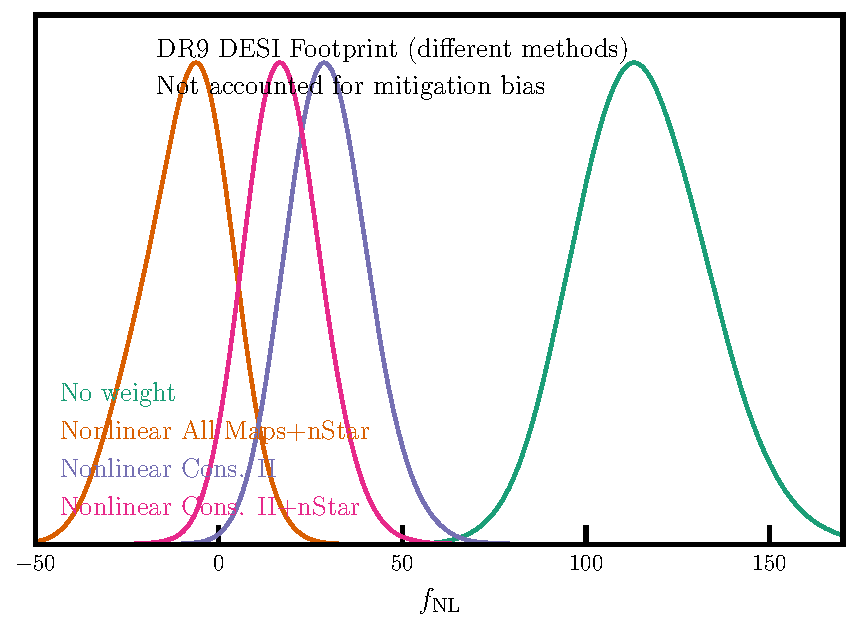
\includegraphics[width=0.45\textwidth]{figures/mcmc_dr9methods1dnoshift.pdf}
    \caption{Same as Figure \ref{fig:mcmc_dr9} but without accouting for over-correction. }
    \label{fig:mcmcdr9noshift}
\end{figure}


\begin{figure}
    \centering
    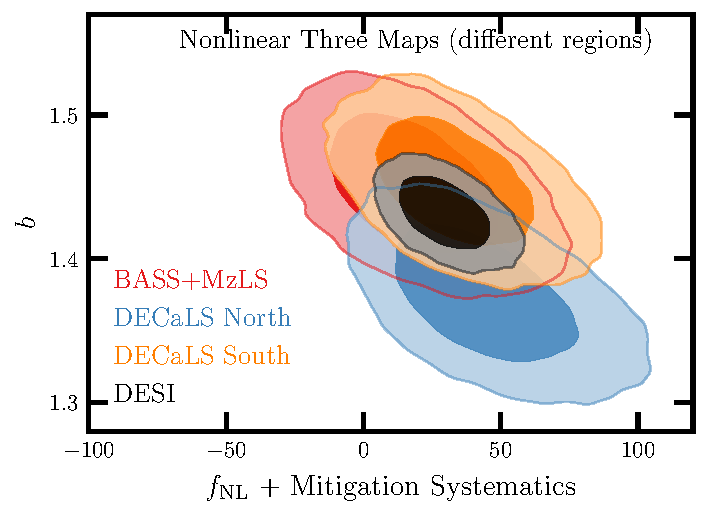
\includegraphics[width=0.45\textwidth]{figures/mcmc_dr9regions.pdf} 
    \caption{The uncalibrated 2D constraints from the DESI LRG targets using the nonlinear nine maps treatment for each imaging survey compared with that for the whole DESI footprint. The dark and light shades represent the $68\%$ and $95\%$ confidence intervals, respectively.}\label{fig:mcmc_dr9reg}
\end{figure}
\begin{figure*}
    \centering
    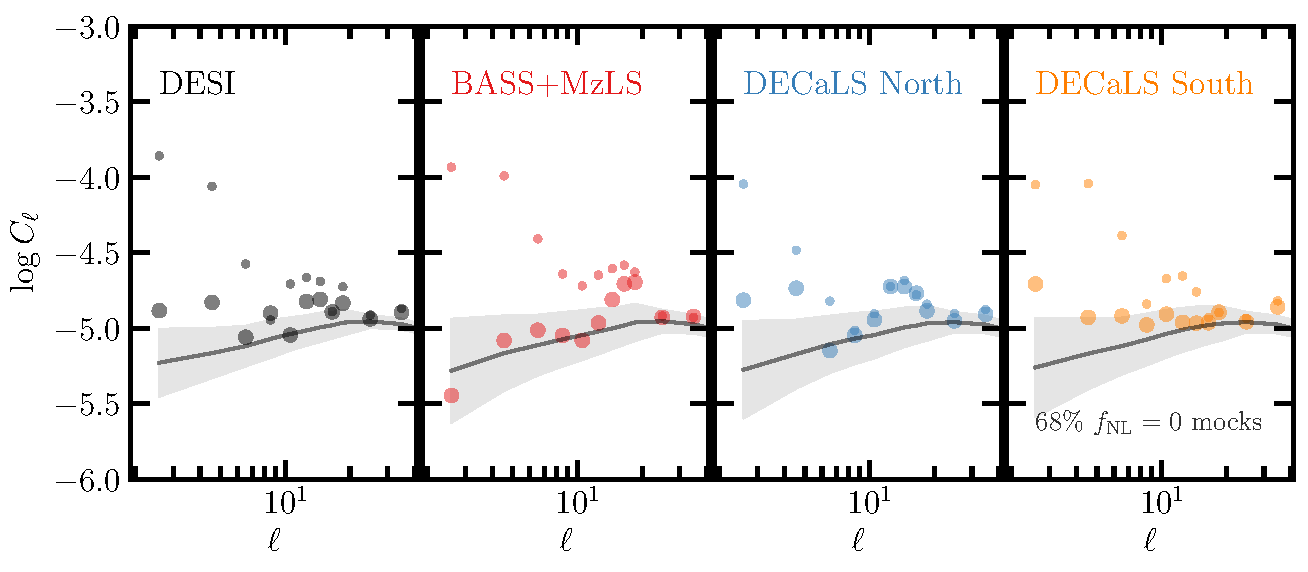
\includegraphics[width=0.9\textwidth]{figures/cldr9_lowell.pdf}
    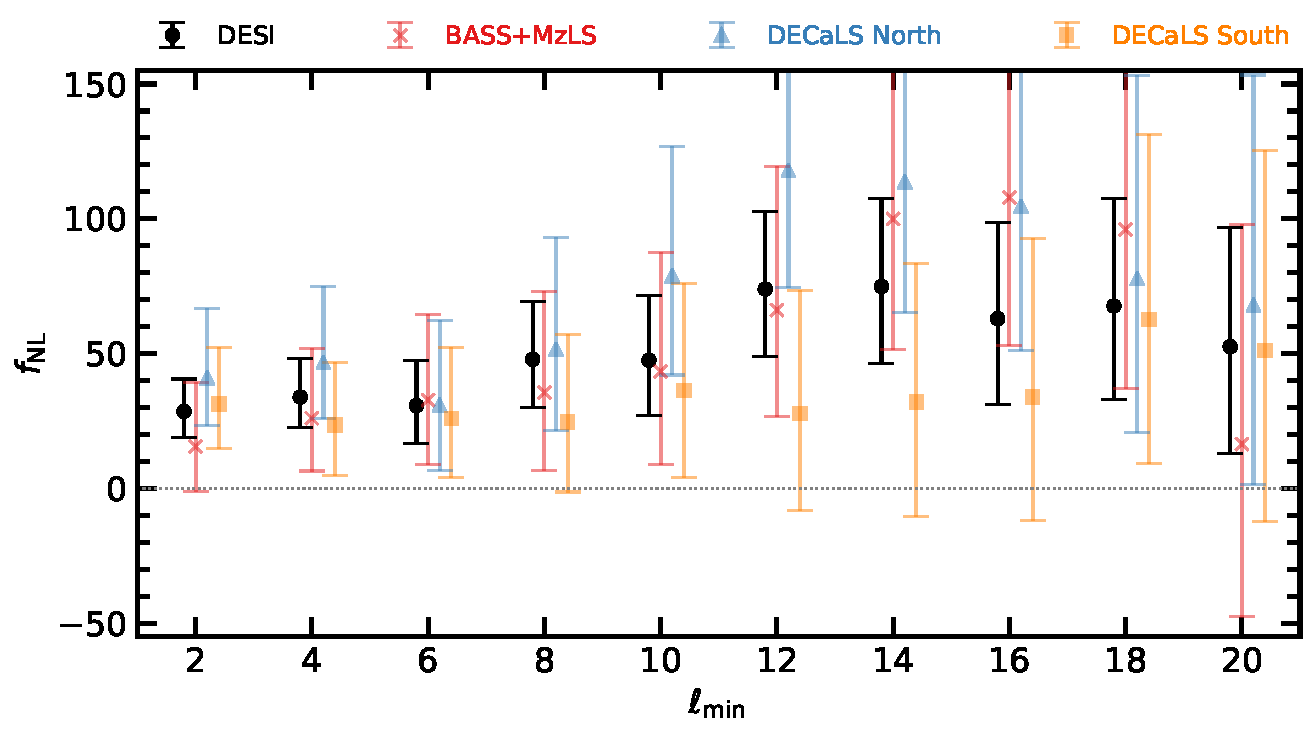
\includegraphics[width=0.9\textwidth]{figures/fnl_elmin.pdf}  
    \caption{Top: The measured power spectrum of the DESI LRG targets before (solid curves) and after \textit{non-linear \mr{nine} maps} (scatter points) for the DESI, BASS+MzLS, DECaLS North, and DECaLS South regions. The solid curve and grey shade respectively represent the mean power spectrum and $68\%$ error from the $\fnl=0$ mocks with the same angular mask for each region. Bottom: The uncalibrated $\fnl$ constraints vs the lowest $\ell$ mode used for fitting $\fnl$. The points represent the best fitting estimates of $\fnl$ and error bars represent $95$\% confidence. The scaling of $\fnl$ is not calibrated to account for over-correction caused by mitigation.}\label{fig:mcmc_dr9elmin}
\end{figure*}


Now we proceed to perform some robustness tests and assess how sensitive the $\fnl$ constraints are to the assumptions made in the analysis or the quality cuts applied to the data. For each case, we re-train the cleaning methods and derive new sets of imaging weights. Accordingly, for the cases where a new survey mask is applied to the data, we re-calculate the covariance matrices using the new survey mask to account for the changes in the survey window and integral constraint effects. Calibrating the mitigation biases for all of these experiments is beyond the scope of this work and redundant, as we are only interested in the relative shift in the $\fnl$ constraints after changing the assumptions. Therefore, the absolute scaling of the $\fnl$ constraints presented here are biased because of the over-correction effect. Table \ref{tab:dr9method} summarizes the uncalibrated $\fnl$ constraints from the DESI LRG targets. Our tests are as follows:

\begin{itemize}[itemindent=*]

\item \textbf{Linear methods}: \mout{Even though the linear three maps approach shows significant remaining systematics (Figure \ref{fig:chi2test} and Table \ref{tab:chi2test}),} \mr{We obtain identical constraints from \textit{linear four maps} and \textit{linear nine maps}, respectively, $20(9)<\fnl<45(58)$ and $19(9)<\fnl<43(57)$ at $68\%(95\%)$ confidence. For the linear treatment methods, the probability of $\fnl$ being greater than zero is $99.9$ per cent. Any attempt to account for the over-correction would elevate this probability even further. The overestimation of $\fnl$ can be attributed to an increase in systematic contamination.}
%
\item \textbf{Imaging regions}: We compare how our constraints from fitting the power spectrum of the whole DESI footprint compares to that from the power spectrum of each imaging region individually, namely BASS+MzLS, DECaLS North, and DECaLS South. Figure~\ref{fig:mcmc_dr9reg} shows the $68\%$ and $95\%$ probability contours on $\fnl$ and $b$ from each individual region, compared with that from DESI. The cleaning method here is \textit{non-linear \mr{nine} maps}, and the covariance matrices are estimated from the $\fnl=0$ mocks. The bias in DECaLS North is lower than the ones from DECaLS South and BASS+MzLS, which might indicate some remaining systematic effects that could not be mitigated with the available imaging systematic maps. This is because given the negative correlation between $b$ and $\fnl$, a larger value of $\fnl$ due to excess clustering power needs to be compensated by a smaller value of $b$. Overall, we find that the constraints from analyzing each imaging survey separately are consistent with each other and DESI within $68\%$ confidence. \mout{Ignoring the over-correction effect, we find that the results from the DECaLS North region to be the only one that finds PNG nonzero at greater than 95\%, which motivates follow-up studies with the spectroscopic sample of LRGs in DECaLS North.}

\item \textbf{Stellar density template (\textit{nStar})}: When not accounting for over-correction, adding the stellar density map appears to result in significant changes in the $\fnl$ constraints, e.g., compare non-linear three maps with non-linear four maps in Table \ref{tab:dr9method}. But these changes disappear when we account for the mitigation bias and we find \mout{all}\mr{both} methods recover the same maximum likelihood estimate for \mr{$\fnl \sim 46$} within $69\%$ confidence, see Table \ref{tab:dr9methodcalib}, which implies that these changes can be associated with the over-correction issue from the chance correlations between the stellar density map and large-scale structure.

\item \textbf{Pixel completeness (\textit{comp. cut})}: We discard pixels with fractional completeness less than half to assess the effect of partially complete pixels on $\fnl$. This pixel completeness cut removes $0.6\%$ of the survey area, and no significant changes in the $\fnl$ constraints are observed.

\item \textbf{Imaging quality (\textit{imag. cut})}: Pixels with poor photometry are removed from our sample by applying the following cuts on imaging; $E[B-V]<0.1$, $nStar < 3000$, ${\rm depth}_{g} > 23.2$, ${\rm depth}_{r} > 22.6$, ${\rm depth}_{z} > 22.5$, ${\rm psfsize}_{g}<2.5$, ${\rm psfsize}_{r}<2.5$, and ${\rm psfsize}_{z}<2$. Although these cuts remove $8\%$ of the survey mask, there is \mout{a negligible}\mr{an insignificant} impact on the best-fitting estimates of $\fnl$ from fitting the DESI power spectrum. However, when each region is fit individually, the BASS+MzLS constraint \mr{is more stable than those from DECaLS North and DECaLS South.} \mout{shift toward higher values of $\fnl$ by approximately $\Delta \fnl \sim 10$, whereas the constraints from the DECaLS North and DECaLS South do not change significantly.} 

\item \textbf{Covariance matrix (\textit{cov})}: We fit the power spectrum of our sample cleaned with \textit{non-linear nine maps} correction, but use the covariance matrix constructed from the $\fnl=76.9$ mocks. With the alternative covariance, a \mr{$7\%$} increase in the 68\% error on $\fnl$, $\sigma(\fnl)$, is observed. We also find that the best-fitting and marginalized mean estimates of $\fnl$ increase slightly by \mr{$\Delta \fnl = 2$}. Overall, we find that the differences are not significant in comparison to the statistical precision.

\item \textbf{External maps (\textit{CALIBZ+HI})}: The neural network \mr{eleven} maps correction includes the additional maps for the neutral column density (HI) and the z-band calibration error (CALIBZ). With this correction, the best-fitting $\fnl$ increases from \mr{$-4$ to $-2$} for DECaLS North and from \mr{$-43$ to $-38$} for DECaLS South, which might suggest that adding HI and CALIBZ increases the input noise, and thus negatively impacts the performance of the neural network model. This test is not performed on BASS+MzLS due to a lack of coverage from the CALIBZ map. 

\item \textbf{Declination mask (\textit{no DEC cut})}: The fiducial mask removes the disconnected islands in DECaLS North and regions with DEC $<-30$ in DECaLS South, where there is a high likelihood of calibration issues as different standard stars are used for photometric calibrations. We analyze our sample without these cuts, and find that the best-fitting and marginalized $\fnl$ mean estimates from DECaLS South shift significantly to higher values of $\fnl$ by \mr{$\Delta \fnl \sim 41$}, which supports the case that there are remaining photometric systematics in the DECaLS South region below DEC $=-30$. On the other hand, the constraints from DECaLS North do not change significantly, indicating the islands do not induce significant contaminations.

\item \textbf{Scale dependence (\textit{varying $\ell_{\rm min}$})}: We raise the value of the lowest harmonic mode $\ell_{\rm min}$ used for the likelihood evaluation during MCMC. This is equivalent to utilizing smaller spatial scales in the measurements of the power spectrum. By doing so, we anticipate a reduction in the impact of imaging systematics on $\fnl$ inference as lower $\ell$ modes are more likely to be contaminated. Figure \ref{fig:mcmc_dr9elmin} illustrates the power spectra before and after the correction with \textit{non-linear \mr{nine} maps} in the top panel. The bottom panel shows the best fitting estimate and $95\%$ error on $\fnl$ with \textit{non-linear nine maps} for the DESI, BASS+MzLS, DECaLS North, and DECaLS South regions. We discover that a slight upward shift in the best fitting estimates of $\fnl$ on scales ranging from $10$ to $20$ for DECaLS North and BASS+MzLS when we utilized a higher $\ell_{\rm min}$. This outcome might imply that the imaging systematic maps do not contain enough information to help the cleaning method null out the contaminating signal in the NGC. We also find that the bump is resilient against an alternative correction, in which we apply the neural networks trained on the DECaLS South to the DECaLS North region (see \ref{ssec:ndecalsbump}). Overall, this result is contrary to what one might predict if a significant systematic-induced spike existed at the very low $\ell$\mr{, or if we had an extremely large-scale systematic leakage from the $\ell=1$ mode}. As a result, it suggests that the underlying issue is more subtle than originally anticipated.
\end{itemize}